\documentclass[journal,10pt,twocolumn]{IEEEtran}

\usepackage{setspace}
\usepackage{gensymb}
\singlespacing
\usepackage[cmex10]{amsmath}

\usepackage{amsthm}

\usepackage{mathrsfs}
\usepackage{txfonts}
\usepackage{stfloats}
\usepackage{bm}
\usepackage{cite}
\usepackage{cases}
\usepackage{subfig}
\usepackage{breqn}
\usepackage{longtable}
\usepackage{multirow}
\usepackage{xfrac}
\usepackage{enumitem}
\usepackage{mathtools}
\usepackage{steinmetz}
\usepackage{tikz}
\usepackage{circuitikz}
\usepackage{verbatim}
\usepackage{tfrupee}
\usepackage[breaklinks=true]{hyperref}
\usepackage{graphicx}
\usepackage{tkz-euclide}
\usepackage{nicefrac}
\usetikzlibrary{calc,math}
\usepackage{listings}
    \usepackage{color}                                            %%
    \usepackage{array}                                            %%
    \usepackage{longtable}                                        %%
    \usepackage{calc}                                             %%
    \usepackage{multirow}                                         %%
    \usepackage{hhline}                                           %%
    \usepackage{ifthen}                                           %%
    \usepackage{lscape}     
\usepackage{multicol}
\usepackage{chngcntr}

\DeclareMathOperator*{\Res}{Res}

\renewcommand\thesection{\arabic{section}}
\renewcommand\thesubsection{\thesection.\arabic{subsection}}
\renewcommand\thesubsubsection{\thesubsection.\arabic{subsubsection}}

\renewcommand\thesectiondis{\arabic{section}}
\renewcommand\thesubsectiondis{\thesectiondis.\arabic{subsection}}
\renewcommand\thesubsubsectiondis{\thesubsectiondis.\arabic{subsubsection}}


\hyphenation{op-tical net-works semi-conduc-tor}
\def\inputGnumericTable{}                                 %%

\lstset{
%language=C,
frame=single, 
breaklines=true,
columns=fullflexible
}
\begin{document}


\newtheorem{theorem}{Theorem}[section]
\newtheorem{problem}{Problem}
\newtheorem{proposition}{Proposition}[section]
\newtheorem{lemma}{Lemma}[section]
\newtheorem{corollary}[theorem]{Corollary}
\newtheorem{example}{Example}[section]
\newtheorem{definition}[problem]{Definition}

\newcommand{\BEQA}{\begin{eqnarray}}
\newcommand{\EEQA}{\end{eqnarray}}
\newcommand{\define}{\stackrel{\triangle}{=}}
\bibliographystyle{IEEEtran}
\raggedbottom
\setlength{\parindent}{0pt}
\providecommand{\mbf}{\mathbf}
\providecommand{\pr}[1]{\ensuremath{\Pr\left(#1\right)}}
\providecommand{\qfunc}[1]{\ensuremath{Q\left(#1\right)}}
\providecommand{\sbrak}[1]{\ensuremath{{}\left[#1\right]}}
\providecommand{\lsbrak}[1]{\ensuremath{{}\left[#1\right.}}
\providecommand{\rsbrak}[1]{\ensuremath{{}\left.#1\right]}}
\providecommand{\brak}[1]{\ensuremath{\left(#1\right)}}
\providecommand{\lbrak}[1]{\ensuremath{\left(#1\right.}}
\providecommand{\rbrak}[1]{\ensuremath{\left.#1\right)}}
\providecommand{\cbrak}[1]{\ensuremath{\left\{#1\right\}}}
\providecommand{\lcbrak}[1]{\ensuremath{\left\{#1\right.}}
\providecommand{\rcbrak}[1]{\ensuremath{\left.#1\right\}}}
\theoremstyle{remark}
\newtheorem{rem}{Remark}
\newcommand{\sgn}{\mathop{\mathrm{sgn}}}
\providecommand{\abs}[1]{\left\vert#1\right\vert}
\providecommand{\res}[1]{\Res\displaylimits_{#1}} 
\providecommand{\norm}[1]{\left\lVert#1\right\rVert}
%\providecommand{\norm}[1]{\lVert#1\rVert}
\providecommand{\mtx}[1]{\mathbf{#1}}
\providecommand{\mean}[1]{E\left[ #1 \right]}
\providecommand{\fourier}{\overset{\mathcal{F}}{ \rightleftharpoons}}
%\providecommand{\hilbert}{\overset{\mathcal{H}}{ \rightleftharpoons}}
\providecommand{\system}{\overset{\mathcal{H}}{ \longleftrightarrow}}
	%\newcommand{\solution}[2]{\textbf{Solution:}{#1}}
\newcommand{\solution}{\noindent \textbf{Solution: }}
\newcommand{\cosec}{\,\text{cosec}\,}
\providecommand{\dec}[2]{\ensuremath{\overset{#1}{\underset{#2}{\gtrless}}}}
\newcommand{\myvec}[1]{\ensuremath{\begin{pmatrix}#1\end{pmatrix}}}
\newcommand{\mydet}[1]{\ensuremath{\begin{vmatrix}#1\end{vmatrix}}}
\numberwithin{equation}{subsection}
\makeatletter
\makeatother
\let\vec\mathbf
\def\putbox#1#2#3{\makebox[0in][l]{\makebox[#1][l]{}\raisebox{\baselineskip}[0in][0in]{\raisebox{#2}[0in][0in]{#3}}}}
     \def\rightbox#1{\makebox[0in][r]{#1}}
     \def\centbox#1{\makebox[0in]{#1}}
     \def\topbox#1{\raisebox{-\baselineskip}[0in][0in]{#1}}
     \def\midbox#1{\raisebox{-0.5\baselineskip}[0in][0in]{#1}}
\vspace{3cm}
\title{Assignment 3}
\author{Gautham Bellamkonda - CS20BTECH11017}
\maketitle
\newpage
\bigskip
\renewcommand{\thetable}{\theenumi}
Download all python codes from 
\begin{lstlisting}
https://github.com/GauthamBellamkonda/AI1103/tree/main/Assignment3/Codes
\end{lstlisting}
and latex-tikz codes from 
\begin{lstlisting}
https://github.com/GauthamBellamkonda/AI1103/tree/main/Assignment3
\end{lstlisting}
\section{Problem}
(GATE 45) Consider a discrete-time channel $Y = X + Z$, where the additive noise $Z$ is signal dependent. In particular, given the transmitted symbol $X \in \{-a, a \}$ at any instant, the noise sample $Z$ is chosen indepedently from a Gaussian distribution with mean $\beta X$ and unit variance. Assume a threshold detector with zero threshold at the receiver. When $\beta = 0$, the BER was found to be $Q(a) = 1 \times 10^{-8}.$
\begin{align}
\left( Q(v) = \dfrac{1}{\sqrt{2 \pi}} \int_v ^{\infty} e^{-\frac{u^2}{2}} du \text{, and for } v > 1 \text{, use } Q(v) = e^{\frac{-v^2}{2}} \right)
\end{align}
When $\beta = -0.3$, BER is closest to
\begin{enumerate}[label = (\Alph*)]
\item $10^{-7}$
\item $10^{-6}$
\item $10^{-4}$ \label{option C}
\item $10^{-2}$
\end{enumerate}
\section{Solution}
Given that $X \in \{ -a, +a\}$ is a random variable.
\begin{align}
\Pr(X=a) &= \dfrac{n(X=a)}{2} = \dfrac{1}{2}\\
\Pr(X=-a) &= \dfrac{n(X=-a)}{2} = \dfrac{1}{2}
\end{align}
Also, $Z$ is chosen from Gaussian Distribution with mean $\beta X$ and unit variance.
\begin{align}
\therefore F_Z(z) &= \text{G} \left( \dfrac{z - \beta X}{1} \right)\\
&= \dfrac{1}{\sqrt{2\pi}}\, \int_{-\infty} ^z \exp \left( \dfrac{-(z-\beta X)^2}{2} \right) dz
\end{align}
On differentiating both the sides with respect to $z$, we get
\begin{align}
f_Z(z) &= \dfrac{d}{dz}F_Z(z) \\
&= \dfrac{d}{dz} \left[ \dfrac{1}{\sqrt{2\pi}}\, \int_{-\infty} ^z \exp \left( \dfrac{-(z-\beta X)^2}{2} \right) dz \right] \\
 &= \dfrac{1}{\sqrt{2\pi}}\,\exp \left(-\frac{(z - \beta X)^2}{2} \right)  \\
\Leftrightarrow f_Y(z + X) &= \dfrac{1}{\sqrt{2\pi}}\,\exp \left(-\frac{(z - \beta X)^2}{2} \right)  \\
\Leftrightarrow f_Y(y) &= \dfrac{1}{\sqrt{2\pi}}\,\exp \left(-\frac{(y - X - \beta X)^2}{2} \right)  \\
&= \dfrac{1}{\sqrt{2\pi}}\,\exp \left(-\frac{(y - X(1 + \beta))^2}{2} \right) \\
\therefore f_Y(y \;|\; X = a) &= \dfrac{1}{\sqrt{2\pi}}\,\exp \left(-\frac{(y - a(1 + \beta))^2}{2} \right) \label{eqn 2.0.9} \\
\& \; f_Y(y \;|\; X = -a) &= \dfrac{1}{\sqrt{2\pi}}\,\exp \left(-\frac{(y + a(1 + \beta))^2}{2} \right) \label{eqn 2.0.10}
\end{align}
Since $X \in \{ -a, +a\}$ is also a random variable,
\begin{align}
f_Y(y) = &f_Y(y\;|\;X = a)\Pr(X=a) \nonumber \\
               &+ f_Y(y\;|\;X = -a)\Pr(X=-a)\\
 = &\dfrac{1}{2} \cdot \dfrac{1}{\sqrt{2\pi}}\,\exp \left(-\frac{(y - a(1 + \beta))^2}{2} \right) \nonumber \\
      &+ \dfrac{1}{2} \cdot \dfrac{1}{\sqrt{2\pi}}\,\exp \left(-\frac{(y + a(1 + \beta))^2}{2} \right)
\end{align}
Therefore, the resultant signal $Y = X+Z$ is comprised of $X$ which can take either positive or negative value, and some noise $Z$. The detector (which has zero threshold) can give us incorrect bits when $X = +a$ and $Y<0$ (BER$_{+a}$) or $X=-a$ and $Y<0$ (BER$_{-a}$), as shown in the graph below.
~\\[-2em]
\begin{figure}[!htb]
    \centering    
	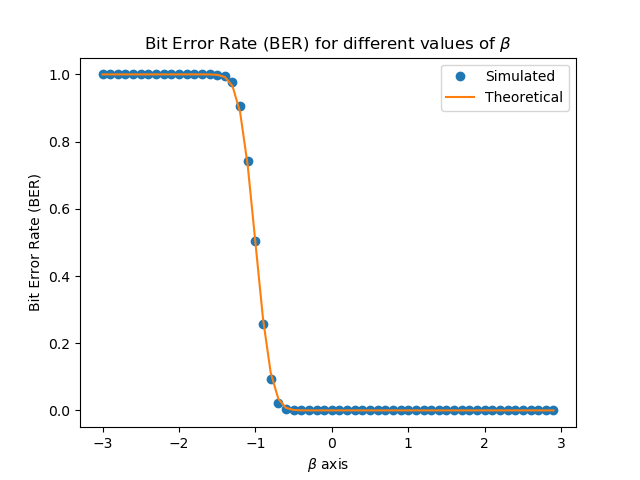
\includegraphics[width=\columnwidth]{./Figures/Figure_1.png}
    \caption{The CDF of $Y$}
\end{figure}
\begin{align}
\therefore \text{BER} = {}& \text{BER}_{+a} + \text{BER}_{-a}\\
= {}& f_Y(y < 0, X = a) + f_Y(y>0, X = -a)\\
 = {}& f_Y(y<0\;|\;X = a) \Pr(X=a) \nonumber \\ &+ f_Y(y>0\;|\;X = -a) \Pr(X=-a)\\
 = {}& \int_{- \infty} ^ 0 \dfrac{1}{2} \cdot f_Y(y\;|\;X = a) dy \nonumber \\
 &+ \int_{0} ^{ \infty} \dfrac{1}{2} \cdot f_Y(y\;|\;X = -a) dy
\end{align}
On substituting the values of $f_Y(y\;|\;X=a)$ and\\
$f_Y(y\;|\;X=-a)$ from \ref{eqn 2.0.9} and \ref{eqn 2.0.10}, 
\begin{align}
\text{BER} = {}& \int_{- \infty } ^ 0 \dfrac{1}{2\sqrt{2\pi}}\,\exp \left(-\frac{(y - a(1 + \beta))^2}{2} \right) dy \nonumber \\
&+ \int_{0} ^ {\infty } \dfrac{1}{2\sqrt{2\pi}}\,\exp \left(-\frac{(y + a(1 + \beta))^2}{2} \right) dy\\
 = {}& \int_{0} ^ {\infty } \dfrac{1}{2\sqrt{2\pi}}\,\exp \left(-\frac{(y + a(1 + \beta))^2}{2} \right) dy \nonumber \\
 &+ \int_{0} ^ {\infty } \dfrac{1}{2\sqrt{2\pi}}\,\exp \left(-\frac{(y + a(1 + \beta))^2}{2} \right) dy\\
 = {}& \int_{0} ^ {\infty } \dfrac{1}{\sqrt{2\pi}}\,\exp \left(-\frac{(y + a(1 + \beta))^2}{2} \right) dy \label{eqn 2.0.19}
\end{align} 
From the definition of $Q(v)$, it is easy to see that the expression in \ref{eqn 2.0.19} is equal to $Q(a(1+\beta))$
\begin{align}
\therefore \text{BER} = Q(a(1+\beta ))
\end{align}
When $\beta = 0$, it is given that 
\begin{align}
\text{BER} = Q(a) &= 10^{-8}
\end{align}
On computing, $Q(1) \approx 0.16$. Since $Q(a)<Q(1)$, it is easy to see that $a>1$ (as $Q(x)$ is a decreasing function)
\begin{align}
\therefore e^{-a^2 / 2} &= 10^{-8}\\
\Leftrightarrow a &\approx 6.069
\end{align}
When $\beta = -0.3$,
\begin{align}
\text{BER} = Q(a(1+\beta)) &= Q(6.069 \times (1-0.3))\\
&= Q(6.069 \times 0.7)\\
&= Q(4.249)\\
&\approx \exp (-\dfrac{4.249^2}{2})\\
&\approx 1.2 \times 10^{-4}
\end{align}
Therefore, when $\beta = -0.3$, BER is closest to $10^{-4}$ and option \ref{option C} is correct.
\end{document}